\chapter{Rocket Analysis}
		A rocket presents a large number of similarities with an inverted pendulum in terms of modeling and control as it will be demonstrated in this chapter. It also adds one degree of freedom compared to the inverted pendulum.
		For the purpose of studying the problem of rocket control, a model rocket was designed and built. Since mechanical design is out of this work's scope, the engineering of this rocket will not be explained, but the CAD files will be available on the GitHub repository.
		
		
		\section{Rocket Description}
			In this section the rocket model will be described to prepare it's modeling.
			This design consists of 2 sections, that will be called here "stages".
			\begin{itemize}
				\item First stage: propulsion
				\begin{itemize}
					\item {A thruster / Solid Rocket Booster (SRB)}
					\item {A thrust vectoring mechanism, also known as gimbal, with two degrees of freedom}
					\item {Two servo motors for actuating the gimbal}
				\end{itemize}
				\item Interstage:
				\begin{itemize}
					\item {An empty fairing separating the propulsion stage from the electronics}
				\end{itemize}
				\item Upper stage: control
				\begin{itemize}
					\item {A frame to hold the electronics}
					\item {A PCB with a micro-controller}
					\item {A plastic separator with anti-vibration bearings}
					\item {On this separator is placed a gyroscope: the attitude sensor}
					\item A nose fairing
				\end{itemize}
			\end{itemize}
			
			
%				\section{Inverted pendulum and rocket}
%			The goal of this section is to demonstrate the similarities between the inverted pendulum and the rocket stabilization processes, and to define a mathematical model and control loop of the behavior of the angle of the rocket body and the angle of the thruster.
%			
%			The purpose of the system is to guarantee a stable flight to the rocket.
%			The modeling of the flight of a rocket can be divided into two equations: velocity and rotation. In this project, the desired trajectory of the rocket flight is considered to be on the zenith axis. This results in a vertical flight, with then a velocity on the same axis as the trajectory.The rocket's rotation is a circular motion on the bottom-to-nose axis. This create a centripetal force.
%			
%			The displacement angle (gimbal angle) is the difference between the actual flight direction, or bottom-to-nose axis, and the zenith axis. Gimbaled thrust are controllable thrusters used to create a torque and reduce the gimbal angle. 
%			
%			In an inverted pendulum, the objective is to keep the stick in horizontal position. The angle difference between the horizontal and the actual axis of the stick is measured in order to then create a compensation torque with the arm. The arm has the same task as the gimbaled thruster, and the horizontal axis is equivalent to the zenith axis.
%			
%			At the desired initial position of the inverted pendulum, the acceleration of the arm is negligible. This implies that the arm only produces a force on the axis going through the center of gravity of the arm and parallel to the lenght of the arm. This is equivalent to the rocket process where the thruster applies a force on the axis going through the center of gravity of the arm and parallel to the lenght of the thruster. 
%			
%			 Sketch of rocket + IP at initial position
%			
%			Therefore the rocket and the inverted pendulum processes are equivalent for a small displacement angle range. The inverted pendulum is then studied in this project as a first approach to the understanding of rocket in-flight stabilization process.
%			
%			The control loop of the rocket system is described in figure ...
%			
%			Figure of closed loop model of rocket
%			
%			The input of the closed loop is the gimbal angle (angle difference between actual flight direction and zenith axis). The output is the new gimbal angle. In the inverted pendulum, the input and output are also the angle differences, between the horizontal and the actual axis of the stick. 
%			
%			By admiting that the inverted pendulum and the rocket processes are similar the equations found in Section 5.2 Modelling of the Arm and Stick can be applied to the rocket, with the rocket body as the stick and the gimbaled thruster as the arm. However the gravity center of the rocket body is not located in its center. Therefore $l_{a}$ and $\frac{l_{s}}{2}$ become respectively $l_{t}$, for the thruster, and $l_{bg}$, for the lenght from the bottom of the rocket body to its center of mass. The equations describing the forces, with $a$ for arm and $s$ for stick respectively replaced by $t$ for thruster and $b$ for rocket body, are:
%			
%			Transfer function as in part "modeling of stick".
		
		\section{Modeling of the rocket body and stick}
			
		The purpose of this section is to have a mathematical model for the different forces applied on the rocket in flight. 
		
		In this project, the trajectory of the rocket is on the zenith axis, or y axis, which implies the impact of the lift on the rocket is negligible. The sum of the forces applied to the rocket in flight can then be described by equation \eqref{eq:F_total}:
		
		\begin{equation}
		F_{total} = m*a = F_{thrust} + F_{drag} - F_{gravity} \si{\newton} \label{eq:F_{total}}
		\end{equation}
		\startexplain
		\explain{$F_{total}$ is the sum of all force}{\si{\newton}}
		\explain{$F_{thrust}$ is the force created by the gimbaled thruster}{\si{\newton}}
		\explain{$F_{drag}$ is the drag force on the rocket}{\si{\newton}}
		\explain{$F_{gravity}$ is the gravity applied on the rocket}{\si{\newton}}
		\stopexplain
		
		The drag force can be expressed by equation \eqref{eq:F_drag}:
		\begin{equation}
		F_{drag} = \frac{1}{2} \cdot C_{d} \cdot \rho \cdot A \cdot v^2 \si{\newton} \label{eq:F_{drag}}
		\end{equation}
		\startexplain
		\explain{$C_{d}$ is the coefficient of drag}{\si{1}}
		\explain{$\rho$ is the air density}{\si{\kilo\gram\per\meter\cubed}}
		\explain{$A$ is the cross sectionnal area of the rocket}{\si{\meter\squared}}
		\explain{$v$ is the velocity of the rocket}{\si{\meter\per\second}}
		\stopexplain
			
		The coefficient of drag and the cross sectionnal area vary depending on the shape of the rocket. Altitude and humidity in the air can impact the air density. Parasit drag can appear due to the surface material or pressure drag.
		
		The gravity force equation is \eqref{eq:F_{gravity}}:
		\begin{equation}
		F_{gravity} = m \cdot g \si{\newton} \label{eq:F_{gravity}}
		\end{equation}
		\startexplain
		\explain{$m$ is the mass of the rocket}{\si{\kilo\gram}}
		\explain{$g$ is the gravitational acceleration}{\si{\meter\per\second\squared}}
		\explain{$A$ is the cross sectionnal area of the rocket}{\si{\meter\squared}}
		\explain{$v$ is the velocity of the rocket}{\si{\meter\per\second}}
		\stopexplain
			
		
		The thrust force is \eqref{eq:F_{thrust}}:
		\begin{equation}
		F_{thrust} = v_{e} \cdot \ddot{m} + A (P_{e} -P_{0}) \si{\newton} \label{eq:F_{thrust}}
		\end{equation}
		\startexplain
		\explain{$v_{e}$ is the velocity of the gimbaled thruster}{\si{\meter\per\second}}
		\explain{$\ddot{m}$ is the mass flow rate}{\si{\kilo\gram\per\second}}
		\explain{$A$ is the nozzle exit area}{\si{\meter\squared}}
		\explain{$P_{e}$ is the pressure of the nozzle exit}{\si{\kilo\gram\per\meter\per\second\squared}}
		\explain{$P_{0}$ is the free stream pressure}{\si{\kilo\gram\per\meter\per\second\squared}}
		\stopexplain
		
		
		The thruster pression and velocity is divided into two equation, respectively ahead and behind the propeller nozzle: $P_{o}$ \eqref{eq:P_{o}} and $P_{e}$ \eqref{eq:P_{e}}.
		
		\begin{equation}
		P_{0} = p_{0} + 0.5 \cdot \rho \cdot(v_{o})^2 \si{\kilo\gram\per\meter\per\second\squared} \label{eq:P_{o}}
		\end{equation}
		\startexplain
		\explain{$p_{o}$ is the static pressure}{\si{\kilo\gram\per\meter\per\second\squared}}
		\explain{$v_{o}$ is the velocity of the rocket}{\si{\meter\per\second}}
		\stopexplain
		
		\begin{equation}
		P_{e} = p_{o} + 0.5 \cdot \rho \cdot(v_{e})^2 \si{\kilo\gram\per\meter\per\second\squared} \label{eq:P_{e}}
		\end{equation}
		\startexplain
		\explain{$v_{e}$ is the exit velocity of the gimbaled thruster}{\si{\meter\per\second}}
		\stopexplain
		
		Therefore, there is three different cases of truster pression:
		\begin{equation}
		P_{e} = P_{a}
		P_{e} > P_{a}
		P_{e} < P_{a}
		\end{equation}
		 insert sketch of the different cases
		 
		
		\startexplain
		\explain{$F_x$ is the force in the x direction}{\si{\newton}}
		\explain{$F_y$ is the force in the y direction}{\si{\newton}}
		\explain{$x_s$ is the position of the center of mass of the stick in the x direction}{\si{\meter}}
		\explain{$y_s$ is the position of the center of mass of the stick in the y direction}{\si{\meter}}
		\explain{$l_t$ is the length of the thruster}{\si{\meter}}
		\explain{$C_g$ is the length between the gimbal and the center of gravity of the rocket}{\si{\meter}}
		\explain{$\theta_t$ is the angle from the thruster to the y-axis}{\si{\radian}}
		\explain{$\theta_b$ is the angle from the rocket body to the y-axis}{\si{\radian}}
		\stopexplain
		All forces, constants and variables that relates to the arm and stick are denoted by a subscripted $a$ and $s$ respectively. 
		
		The behaviour of the stick can be fully described by three movements; two translatory and one rotary. It can move in the x and y direction and rotate around it's own axis.
		
		%To find the relation between the angles, the free body diagram of the joint of the arm and stick is made on \autoref{fig:freebodystick}.
		%\begin{figure}[htbp]
		%\centering
		%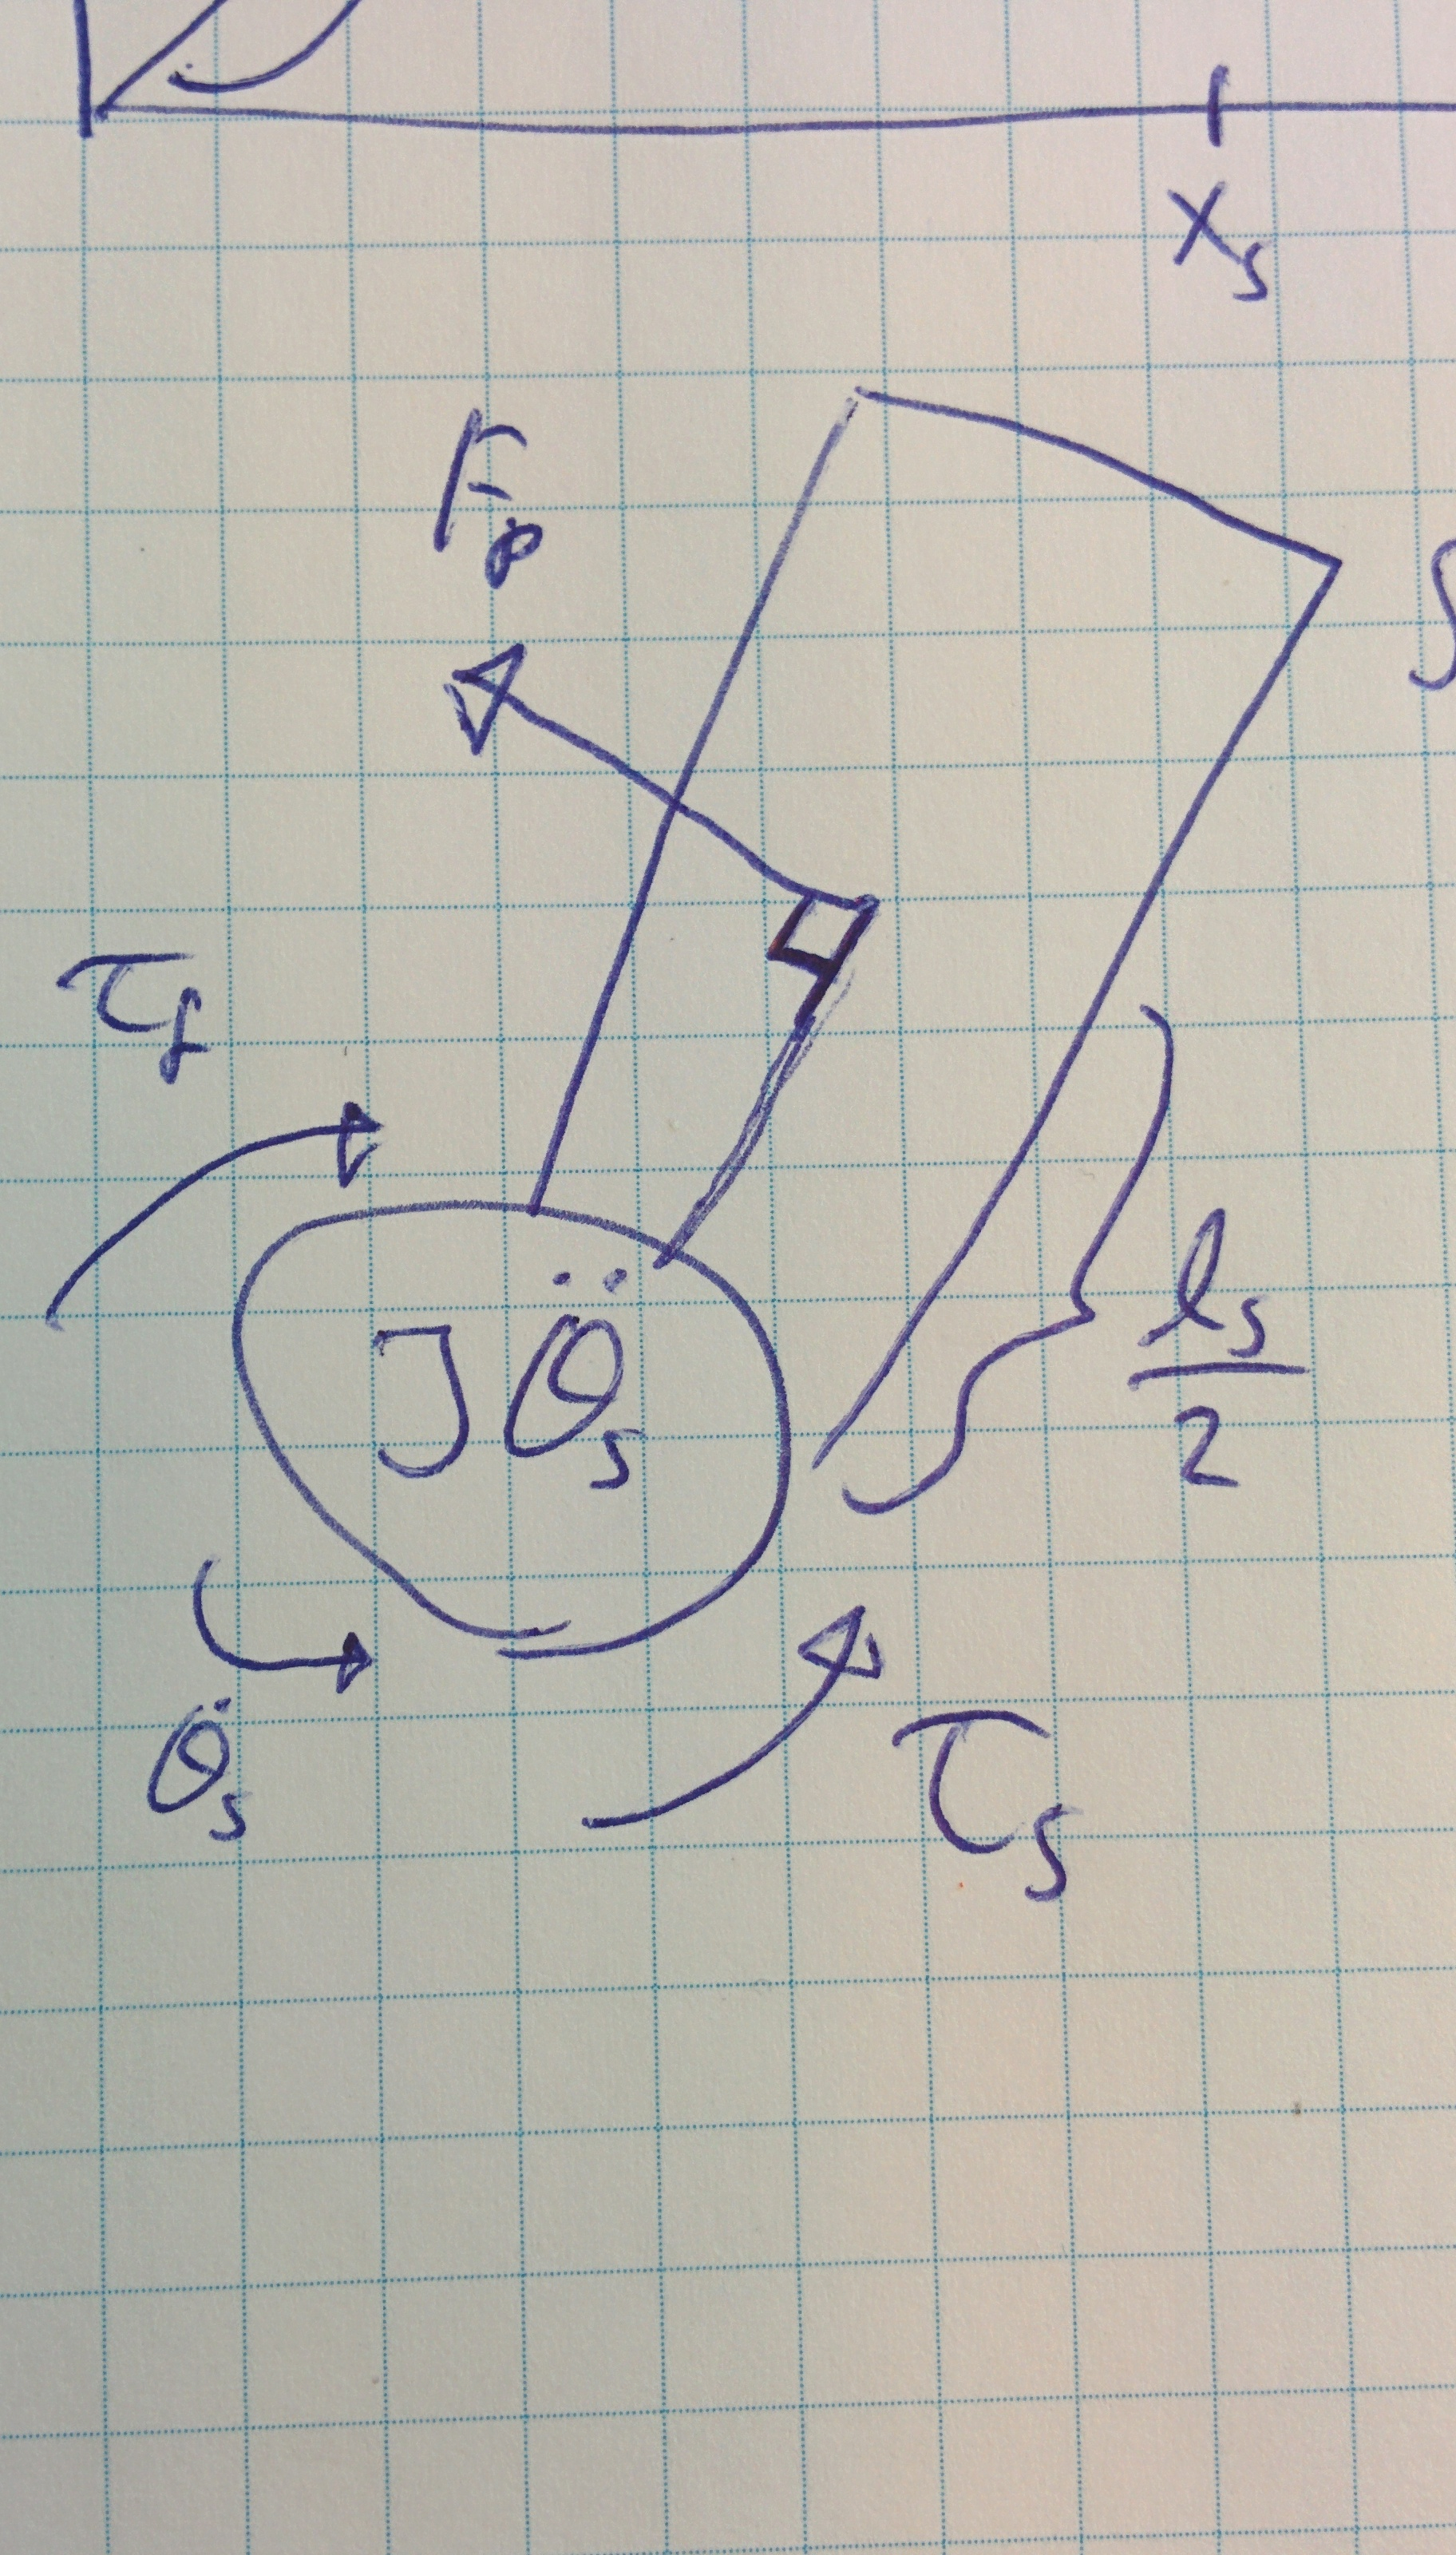
\includegraphics[width=0.25\textwidth]{FreeBodyPendulum}
		%\caption{Free body diagram of the joint that connects the arm and the stick.}
		%\label{fig:freebodystick}
		%\end{figure}
		%\todo[inline, author=Jacob]{Make pretty graph}
		%
		%The moment of inertia for the joint is described by \autoref{eq:Jrthetas}.
		%\begin{subequations}
		%\begin{flalign}
		%& J_r\ddot{\theta}_s=\tau_s-\tau_f  \label{eq:Jrthetas} \\
		%& \tau_s =F_p\frac{l_s}{2} \\
		%& \tau_f =b_{as}\dot{\theta}_{as} 
		%\end{flalign}
		%\end{subequations}
		%\startexplain
		%	\explain{$J_r$ is the moment of inertia for the stick}{\si{\kg\square\meter}}
		%	\explain{$\ddot{\theta}_s$ is the angular acceleration of the stick}{\si{\radian\per\square\second}}
		%	\explain{$\tau_s$ is the torque induced by the rotation of the stick}{\si{\newton\meter}}
		%	\explain{$\tau_f$ is the torque of the friction acting on the stick}{\si{\newton\meter}}
		%	\explain{$F_p$ is the force perpendicular to the stick at the center of mass}{\si{\newton}}
		%	\explain{$b_{as}$ is the viscous friction coefficient between the arm and the stick}{\si{\newton\meter\second}}
		%	\explain{$\dot{\theta}_{as}$ is the difference in angular velocity between the arm and the stick ($\dot{\theta}_s-\dot{\theta}_a$)}{\si{\radian\per\second}}
		%\stopexplain
		%
		%The friction is calculated from the difference in angular velocity as the stick could be perfectly upright while the arm moves causing the joint to turn. The angle of the arm is not considered as producing a torque acting on the joint but as part of the force on the stick, $F_p$.
		
		The forces acting on the rocket in the x and y directions are found by \autoref{eq:FxFy} using Newton's 2nd law of motion. Unlike in the inverted pendulum, there is no reaction to gravity from the arm, thus gravity doesn't produce any torque.
		
		\begin{subequations}  \label{eq:FxFy}
			\begin{flalign}
				& F_x=\ddot{x}_sM_s  \\
				& F_y=\ddot{y}_sM_s  \\
			\end{flalign}
		\end{subequations}
		\startexplain
		\explain{$M_s$ is the mass of the stick}{\si{\kilo\gram}}
		\stopexplain
		The position of the center of mass of the rocket in the x and y direction is found by \autoref{eq:xsys} using geometry.
		\begin{subequations}\label{eq:xsys} 
			\begin{flalign}
				& x_s=l_t\sin (-\theta_t)+C_g \sin (-\theta_b) \\
				& x_s=-l_t\sin (\theta_t)-C_g \sin (\theta_b) \\
				& y_s = l_t\cos (-\theta_t)+C_g \cos(-\theta_b) \\
				& y_s = l_t\cos (\theta_t)+C_g \cos(\theta_b) 
			\end{flalign}
		\end{subequations}
		
		The derivatives of $x_s$ and $y_s$ is found in \autoref{eq:diffxy}.
		\begin{subequations}\label{eq:diffxy} 
			\begin{flalign}
				\hspace{30pt} & \dot{x}_s=-l_t\dot{\theta}_a\cos(\theta_t)-C_g\dot{\theta}_s\cos(\theta_b) & [\si{\meter\per\second}] \\
				& \ddot{x}_s=-l_t\ddot{\theta}_a\cos(\theta_t)+l_t\dot{\theta}_a^2\sin(\theta_t)-C_g\ddot{\theta}_s\cos(\theta_b)+C_g\dot{\theta}_s^2\sin(\theta_b) & [\si{\meter\per\square\second}] \\
				& \dot{y}_s=-l_t \dot{\theta}_a\sin(\theta_t)-C_g\dot{\theta}_s\sin(\theta_b) & [\si{\meter\per\second}] \\
				& \ddot{y}_s=-l_t\ddot{\theta}_a\sin(\theta_t)-l_t\dot{\theta}_a^2\cos(\theta_t)-C_g\ddot{\theta}_s\sin(\theta_b)-C_g\dot{\theta}_s^2\cos(\theta_b) & [\si{\meter\per\square\second}]
			\end{flalign}
		\end{subequations}
		
		The forces $F_x$ and $F_y$ can be decomposed into perpendicular and parallel forces at that point. The parallel forces are negligible when assuming the stick is perfectly solid and unable to stretch or compress. The perpendicular forces is found by \autoref{eq:perpFxFy} and are seen on \autoref{fig:ArmStick}.
		
		%\begin{figure}[htbp]
		%\centering
		%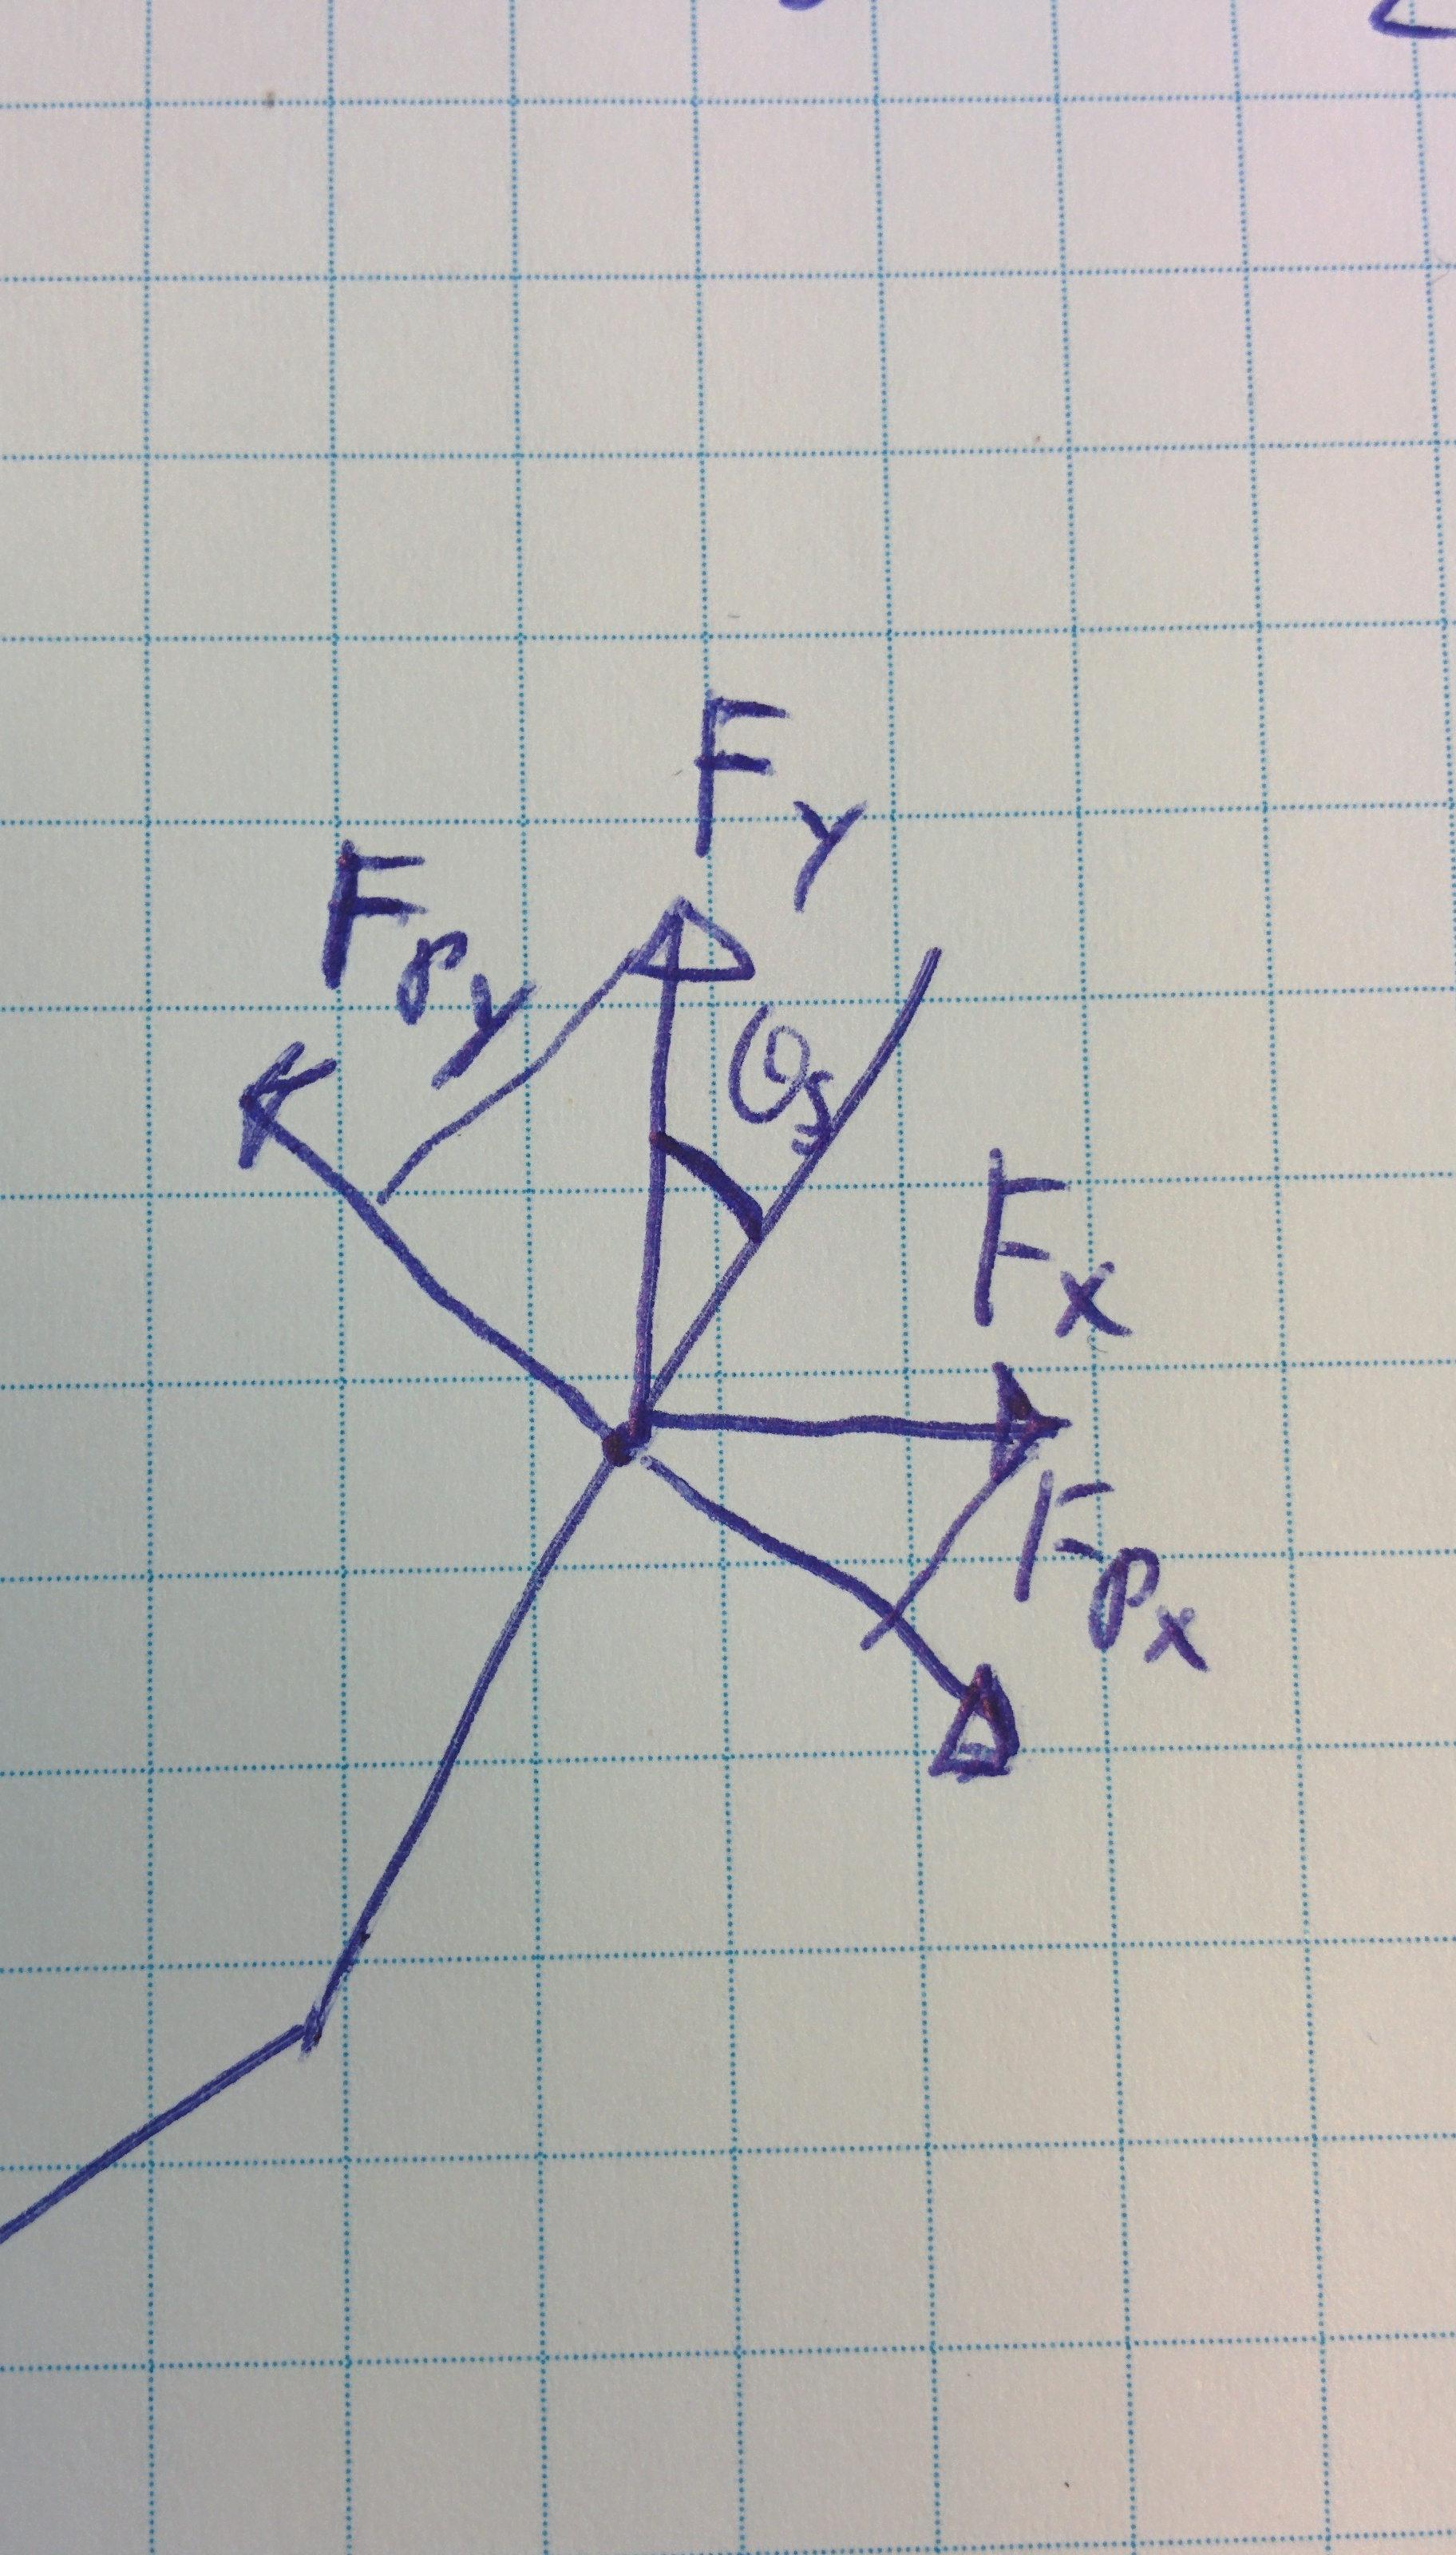
\includegraphics[width=0.25\textwidth]{ForcePerp}
		%\caption{Diagram of the forces, $F_x$ and $F_y$, decomposed into perpendicular forces.}
		%\label{fig:ForcePerp}
		%\end{figure}
		
		\begin{subequations}\label{eq:perpFxFy}
			\begin{flalign}
				& F_{px}=F_x\cos(\theta_b) \\
				& F_{py}=F_y\sin(\theta_b)  \\
				& F_p = F_{px}+F_{py} 
			\end{flalign}
		\end{subequations}
		
		The rotary force of the stick is described by \autoref{eq:JrLong}.
		\begin{subequations}
			\begin{flalign}
				J_r\ddot{\theta}_s &=C_g\left(F_x\cos(\theta_b)+F_y\sin(\theta_b)\right)-b_{as}\dot{\theta}_{as}  \\
				J_r\ddot{\theta}_s = C_g \cdot M_s \Big( &-l_t\ddot{\theta}_a\left(\cos(\theta_t)\cos(\theta_b)+\sin(\theta_t)\sin(\theta_b)\right) \notag \\
				& +l_t\dot{\theta}_a^2\left(\sin(\theta_t)\cos(\theta_b)-\cos(\theta_t)\sin(\theta_b)\right) \notag \\
				& -C_g\ddot{\theta}_s\left(\cos(\theta_b)\cos(\theta_b)+\sin(\theta_b)\sin(\theta_b)\right) \notag \\
				& +C_g\dot{\theta}_s^2\left(\sin(\theta_b)\cos(\theta_b)-\cos(\theta_b)\sin(\theta_b)\right)  \notag \Big)-b_{as}\dot{\theta}_{as} \label{eq:JrLong}
			\end{flalign}
		\end{subequations}
		
		Using the trigonometric properties in \autoref{eq:trigprop}, \autoref{eq:JrLong} is reduced to \autoref{eq:JrShort}.
		\begin{subequations} \label{eq:trigprop}
			\begin{flalign}
				& \cos(\theta_t)\cos(\theta_b)\pm \sin(\theta_t)\sin(\theta_b)=\cos(\theta_t \mp \theta_b)  \\
				& \sin(\theta_t)\cos(\theta_b)\pm \cos(\theta_t)\sin(\theta_b) = \sin(\theta_t \pm \theta_b) \\ 
				& \cos(\theta_b)^2+\sin(\theta_b)^2=1 
			\end{flalign}
		\end{subequations}
		\begin{flalign}
			J_r\ddot{\theta}_s = C_gM_s \Big( &-l_t\ddot{\theta}_a \cos(\theta_t-\theta_b)+l_t\dot{\theta}_a^2 \sin(\theta_t-\theta_b) \notag \\
			&-C_g\ddot{\theta}_s \Big)-b_{as}\dot{\theta}_{as} \label{eq:JrShort}
		\end{flalign}
		
		This is the nonlinear mathematical model for the system. This will be linearized in order to perform a Laplace transformation. The linearization is made with a 1st order Taylor approximation. The linearization is done at the equilibrium point where the arm is in an upright position i.e. $\theta_b=0$. In the equilibrium point the derivatives of all the inputs and outputs are 0. In this case the inputs and outputs are $\theta_t$ and $\theta_b$ and the operating point is $\bar{\theta}_a=0$ and $\bar{\theta}_s=0$. The nonlinear model is expressed as a function of the inputs and outputs as seen in \autoref{eq:nonlinearmodel}.
		\begin{flalign}\label{eq:nonlinearmodel}
			f\left(\theta_t, \dot{\theta}_a, \ddot{\theta}_a, \theta_b, \ddot{\theta}_s\right)=C_gM_s \Big( &-l_t\ddot{\theta}_a \cos(\theta_t-\theta_b)+l_t\dot{\theta}_a^2 \sin(\theta_t-\theta_b) \notag \\
			&-C_g\ddot{\theta}_s \Big)-b_{as}\dot{\theta}_{as}-J_r\ddot{\theta}_s
		\end{flalign}
		
		Generally all equilibriums can be found by setting \autoref{eq:nonlinearmodel} equal to 0 and the derivatives to 0 and solving for $\theta_t=\bar{\theta}_a$ and $\theta_b=\bar{\theta}_s$. For the pendulum it's easy to see the only two equilibriums are the stick pointing straight up and straight down. 
		
		The 1st order Taylor approximation of an equation with multiple variables is seen in \autoref{eq:1stTaylor}.
		\begin{flalign}
			f\left(\theta_t, \dot{\theta}_a, \ddot{\theta}_a, \theta_b, \ddot{\theta}_s\right) & \approx f\left(\bar{\theta}_a, 0, 0, \bar{\theta}_s, 0\right) + \left. \frac{\partial f}{\partial \theta_t}\right|_{(\bar{\theta}_a, \bar{\theta}_s)} \hat{\theta}_a \notag \\
			& \phantom{=} + \left. \frac{\partial f}{\partial \dot{\theta}_a}\right|_{(\bar{\theta}_a, \bar{\theta}_s)} \hat{\dot{\theta}}_a + \left. \frac{\partial f}{\partial \ddot{\theta}_a}\right|_{(\bar{\theta}_a, \bar{\theta}_s)} \hat{\ddot{\theta}}_a \notag \\
			& \phantom{=} + \left. \frac{\partial f}{\partial \theta_b}\right|_{(\bar{\theta}_a, \bar{\theta}_s)} \hat{\theta}_s + \left. \frac{\partial f}{\partial \ddot{\theta}_s}\right|_{(\bar{\theta}_a, \bar{\theta}_s)} \hat{\ddot{\theta}}_s \label{eq:1stTaylor}
		\end{flalign}
		\startexplain
		\explain{$\bar{\theta}$ denotes the angle in an operating point}{\si{\radian}}
		\explain{$\hat{\theta}$ denotes the angle of the small signal variances}{\si{\radian}}
		\stopexplain
		
		The 3 terms with sin or cos in \autoref{eq:JrShort} will be approximated individually using \autoref{eq:1stTaylor}, remembering that $\bar{\theta}=\bar{\dot{\theta}}=\bar{\ddot{\theta}}=0$ in the equilibrium.
		\begin{subequations}
			\begin{flalign}
				-l_t\ddot{\theta}_a\cos\left(\theta_t-\theta_b\right)  \approx & \ 0 + l_t\bar{\ddot{\theta}}_a\sin\left(\bar{\theta}_a-\bar{\theta}_s\right)\hat{\theta}_a  \notag \\ 
				& -l_t\cos\left(\bar{\theta}_a-\bar{\theta}_s\right)\hat{\ddot{\theta}}_a - l_t\bar{\ddot{\theta}}_a\sin\left(\bar{\theta}_a-\bar{\theta}_s\right)\hat{\theta}_s   \\
				-l_t\ddot{\theta}_a\cos\left(\theta_t-\theta_b\right) \approx &-l_t\hat{\ddot{\theta}}_a 
			\end{flalign} %\bar{\ddot{\theta}}_s
		\end{subequations}
		\begin{subequations}
			\begin{flalign}
				l_t\dot{\theta}_a^2\sin\left(\theta_t-\theta_b\right)  \approx &\ 0 + l_t\bar{\dot{\theta}}_a^2\cos\left(\bar{\theta}_a-\bar{\theta}_s\right)\hat{\theta}_a  \notag \\
				& + 2l_t\bar{\dot{\theta}}_a\sin\left(\bar{\theta}_a-\bar{\theta}_s\right)\hat{\dot{\theta}}_a-l_t\bar{\dot{\theta}}_a^2\cos\left(\bar{\theta}_a-\bar{\theta}_s\right)\hat{\theta}_s   \\
				l_t\dot{\theta}_a^2\sin\left(\bar{\theta}_a-\bar{\theta}_s\right) \approx & \ 0 
			\end{flalign}
		\end{subequations}
		
		Inserting the linearized terms in \autoref{eq:JrShort} and using the moment of inertia for a rotating stick, $J_r=\frac{1}{12}M_sl_s^2$, the linearized model becomes \eqref{eq:JrFinal}.
		\begin{subequations}
			\begin{flalign}
				& \frac{1}{12}M_sl_s^2\hat{\ddot{\theta}}_s= M_s\left(-l_t\hat{\ddot{\theta}}_a-C_g\hat{\ddot{\theta}}_s+g\hat{\theta}_s\right)-b_{as}\hat{\dot{\theta}}_{as}   \\
				& \frac{1}{12}M_sl_s^2\hat{\ddot{\theta}}_s+\frac{1}{4}M_sl_s^2\hat{\ddot{\theta}}_s=C_gM_s\left(-l_t\hat{\ddot{\theta}}_a+g\hat{\theta}_s\right)-b_{as}\hat{\dot{\theta}}_{as}   \\
				& \frac{1}{3}M_sl_s^2\hat{\ddot{\theta}}_s=C_gM_s\left(-l_t\hat{\ddot{\theta}}_a+g\hat{\theta}_s\right)-b_{as}\hat{\dot{\theta}}_{as}  \label{eq:TauSmLin} \\
				& \hat{\ddot{\theta}}_s=\frac{3}{2l_s}\left(-l_t\hat{\ddot{\theta}}_a+g\hat{\theta}_s\right)-\frac{3b_{as}\left(\hat{\dot{\theta}}_s-\hat{\dot{\theta}}_a\right)}{M_sl_s^2} \label{eq:JrFinal}
			\end{flalign}
		\end{subequations}
		
		The linearized model is now Laplace transformed in \autoref{eq:tfArmStick} in order to find the transfer function.
		\begin{subequations}
			\begin{flalign}
				& s^2\Theta_s=\frac{3}{2l_s}\left(-s^2l_t\Theta_a+g\Theta_s\right)-s\frac{3b_{as}}{M_sl_s^2}\Theta_s+s\frac{3b_{as}}{M_sl_s^2}\Theta_a  \\
				& \Theta_s\left(s^2+\frac{3b_{as}}{M_sl_s^2}s-\frac{3g}{2l_s}\right)=\Theta_a\left(-\frac{3l_t}{2l_s}s^2+\frac{3b_{as}}{M_sl_s^2}s\right)  \\
				& \frac{\Theta_s}{\Theta_a}=-\frac{\frac{3l_t}{2l_s}s^2-\frac{3b_{as}}{M_sl_s^2}s}{s^2+\frac{3b_{as}}{M_sl_s^2}s-\frac{3g}{2l_s}} \label{eq:tfArmStick}
			\end{flalign}
		\end{subequations}
		
		A linearized model in the Laplace domain for the arm and the stick has been derived and the model for the gears is now derived.



